\documentclass[mathNotesPreamble]{subfiles}
\begin{document}
%\relscale{1.4} %TODO
\section{14.5: Curvature and Normal Vectors:}

  There are two ways to change the velocity, or in other words, to accelerate:
  \begin{itemize}
    \item 
      change in speed
    \item 
      change in direction 
  \end{itemize}
  The change in direction is referred to as \textit{curvature}. Recall that if we have a smooth curve $\vecr(t)$, the unit tangent vector is
    \[\vecT(t)=\frac{\vecr'(t)}{\abs{\vecr'(t)}}=\frac{\vecv(t)}{\abs{\vecv(t)}}\]

  Specifically, \textit{curvature} of the curve is the magnitude of the rate at which $\vecT$ changes with respect to arc length.
  \vspace*{\stretch{1}}

  \begin{center}
    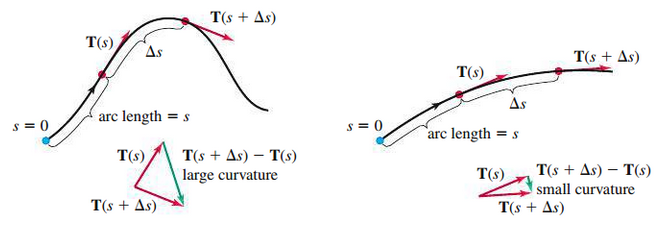
\includegraphics[width=0.8\linewidth]{images/briggs_14_05/fig14_29}
  \end{center}
  \vspace*{\stretch{1}}

  \begin{defn*}[Curvature]
    Let $\vecr$ describe a smooth parameterized curve. If $s$ denotes arc length and $\vecT=\vecr'/\abs{\vecr'}$ is the unit tangent vector, the \textbf{curvature} is $\ds\kappa(s)=\abs{\frac{d\vecT}{ds}}$.
  \end{defn*}
  \pagebreak

  \noindent
  \fbox{\parbox{0.9875\linewidth}{
    \textbf{Theorem 14.4: Curvature Formula}\\
    Let $\vecr(t)$ describe a smooth parameterized curve, where $t$ is any parameter. If $\vecv=\vecr'$ is the velocity and $\vecT$ is the unit tangent vector, then the curvature is
      \[\kappa(t)=\frac{1}{\abs{\vecv}}\abs{\frac{d\vecT}{dt}}=\frac{\abs{\vecT'(t)}}{\abs{\vecr'(t)}}.\]
  }}
  \begin{itemize}
    \item 
      $\kappa$ is a non-negative scalar-valued function
    \item 
      Curvature of zero corresponds to a straight line
    \item 
      A relatively flat curve has a small curvature
    \item 
      A tight curve has a larger curvature
  \end{itemize}

  \begin{ex*}
    Consider the line
      \[\vecr(t)=\bracket{x_0+at,\,y_0+bt,\,z_0+ct},\textnormal{ for }-\infty<t<\infty.\]
    Compute $\kappa$.
  \end{ex*}

  \pagebreak

  \begin{ex*}
    Consider the circle
      \[\vecr(t)=\bracket{R\cos(t),\,R\sin(t)}\]
    for $0\leq t\leq 2\pi$, where $R>0$. Show that $\kappa=1/R$.
  \end{ex*}
  \vspace*{\stretch{1}}

  \begin{ex*}
    Consider the curve
      \[\vecr(t)=\bracket{2\cos(t),\,2\sin(t),\,\sqrt{5}t}\]
    Compute $\kappa$.
  \end{ex*}
  \vspace*{\stretch{1}}

  \pagebreak
  \textbf{An Alternative Curvature Formula:}\\
  Consider a smooth function $\vecr(t)$ with non-zero velocity $\vecv(t)=\vecr'(t)$ and non-zero acceleration $\veca(t)=\vecv'(t)$. 
    \[\vecT=\frac{\vecv}{\abs{\vecv}}\ \Rightarrow\   \vecv=\abs{\vecv}\,\vecT.\]
  Thus
    \[\veca=\frac{d\vecv}{dt}=\ddt\sbrkt{\abs{\vecv}\,\vecT}=\ddt\sbrkt{\abs{\vecv}}\,\vecT+\abs{\vecv}\,\frac{d\vecT}{dt}.\]
  Now we form $\vecv\times\veca$:
  \begin{align*}
    \vecv\times\veca&=\abs{\vecv}\,\vecT\times\parens{\ddt\sbrkt{\abs{\vecv}}\,\vecT+\abs{\vecv}\,\frac{d\vecT}{dt}}\\[5pt]
      &=\underbrace{\abs{\vecv}\,\vecT\times\ddt\sbrkt{\abs{\vecv}}\,\vecT}_{\bfO}+\abs{\vecv}\,\vecT\times\abs{\vecv}\,\frac{d\vecT}{dt}
  \end{align*}
  Since $\vecT$ is a unit vector, $\vecT$ and $d\vecT/dt$ are orthogonal (Theorem 14.2). Thus
  \begin{align*}
    \abs{\vecv\times\veca}=\abs{\abs{\vecv}\,\vecT\times\abs{\vecv}\,\frac{d\vecT}{dt}}=\abs{\vecv}\underbrace{\abs{\vecT}}_1\,\abs{\abs{\vecv}\frac{d\vecT}{dt}}\underbrace{\sin\theta}_1
      =\abs{\vecv}^2 \abs{\frac{d\vecT}{dt}}
  \end{align*}
  Now, using Theorem 14.4, where $\ds\abs{\frac{d\vecT}{dt}}=\kappa \abs{\vecv}$, we have
    \[\abs{\vecv\times\veca}=\abs{\vecv}^2\abs{\frac{d\vecT}{dt}}=\abs{\vecv}^2\,\kappa\abs{\vecv}=\kappa\abs{\vecv}^3.\]

  \vspace*{\stretch{1}}
  \noindent
  \fbox{\parbox{0.9875\linewidth}{
    \textbf{Theorem 14.5: Alternative Curvature Formula}\\
    Let $\vecr$ be the position of an object moving on a smooth curve. The \textbf{curvature} at a point on the curve is
      \[\kappa=\frac{\abs{\vecv\times\veca}}{\abs{\vecv}^3},\]
    where $\vecv=\vecr'$ is the velocity and $\veca=\vecv'$ is the acceleration.
  }}

  \pagebreak

  \begin{ex*}
    Consider the curve
      \[\vecr(t)=\bracket{-16\cos(t),\,16\sin(t),\,0}.\]
    Compute the curvature $\kappa$ using both methods.
  \end{ex*}

  \pagebreak
  \textbf{Principal Unit Normal Vector}\\
  Curvature indicates how quickly a curve turns. The principal unit normal vector determines the \textit{direction} in which a curve turns.

  \begin{defn*}[Principal Unit Normal Vector]
    Let $\vecr$ describe a smooth curve parameterized by arc length. The \textbf{principal unit normal vector} at a point $P$ on the curve at which $\kappa\neq 0$ is
      \[\vecN(s)=\frac{d\vecT/ds}{\abs{d\vecT/ds}}=\frac{1}{\kappa}\frac{d\vecT}{ds}.\]
    For other parameters, we use the equivalent formula
      \[\vecN(t)=\frac{d\vecT/dt}{\abs{d\vecT/dt}},\]
    evaluated at the value of $t$ corresponding to $P$.
  \end{defn*}
  \begin{center}
    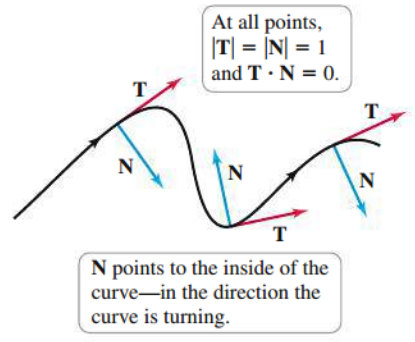
\includegraphics[width=0.275\linewidth]{images/briggs_14_05/fig14_31}
  \end{center}

  \noindent
  \fbox{\parbox{0.9875\linewidth}{
    \textbf{Theorem 14.6: Properties of the Principal Unit Normal Vector}\\
    Let $\vecr$ describe a smooth parameterized curve with unit tangent vector $\vecT$ and principal unit normal vector $\vecN$.
    \begin{enumerate}
      \item 
        $\vecT$ and $\vecN$ are orthogonal at all points of the curve; that is, $\vecT\cdot\vecN=0$ at all points where $\vecN$ is defined.
      \item 
        The principal unit normal vector points to the inside of the curve -- in the direction that the curve is turning.
    \end{enumerate}
  }}
  \pagebreak

  \begin{ex*}
    For the curve $\vecr(t)=\bracket{a\cos(t),\,a\sin(t),\,bt}$, find the unit tangent vector $\vecT$ and the principal unit normal vector $\vecN$. Verify $\abs{\vecT}=\abs{\vecN}=1$ and $\vecT\cdot\vecN=0$.
  \end{ex*}

  \pagebreak

  \textbf{Components of the Acceleration}\\
  Recall that the change in velocity, or acceleration, of an object can change in \textit{speed} (in the direction of $\vecT$) and in \textit{direction} (in the direction of $\vecN$).
  $\ds\vecT=\frac{\vecv}{\abs{\vecv}} \Longrightarrow \vecv=\vecT\abs{\vecv}=\vecT\,\frac{ds}{dt}$.
  \vspace*{\stretch{1}}

  \begin{align*}
    \veca= \frac{d\vecv}{dt}&=\ddt\parens{\vecT\frac{ds}{dt}}\\
      &=\frac{d\vecT}{dt}\,\frac{ds}{dt}+\vecT\frac{d^2s}{dt^2}\\
      &=\underbrace{\frac{d\vecT}{ds}}_{\kappa \vecN}\underbrace{\frac{ds}{dt}}_{\abs{\vecv}}\,\underbrace{\frac{ds}{dt}}_{\abs{\vecv}}+\vecT \frac{d^2s}{dt^2}\\
      &=\kappa\abs{\vecv}^2\, \vecN+\frac{d^2s}{dt^2}\,\vecT.
  \end{align*}   
  \vspace*{\stretch{1}}
  
  \noindent
  \fbox{\parbox{0.9875\linewidth}{
    \textbf{Theorem 14.7: Tangential and Normal Components of the Acceleration}\\
    The acceleration vector of an object moving in space along a smooth curve has the following representation in terms of its \textbf{tangential component} $a_T$ (in the direction of $\vecT$) and its \textbf{normal component} $a_N$ (in the direction of $\vecN$):
      \[\veca=a_N\vecN+a_T\vecT,\]
    where $a_N=\kappa\abs{\vecv}^2=\ds\frac{\abs{\vecv\times\veca}}{\abs{\vecv}}$ and $a_T=\ds\frac{d^2s}{dt^2}$.
  }}
  \pagebreak

  \begin{ex*}
    Consider the function
      \[\vecr(t)=\bracket{-2t+2,\,-2t+3,\,-2t+2}.\]
    Find the tangential and normal components of the acceleration.
  \end{ex*}
  \vspace*{\stretch{1}}

  \begin{ex*}
    Find the components of the acceleration on the circular trajectory
      \[\vecr(t)=\bracket{R\cos(\omega t),\,R\sin(\omega t)}.\]
  \end{ex*}
  \vspace*{\stretch{1}}
  \pagebreak

  \begin{ex*}
    The driver of a car follows the parabolic trajectory $\vecr(t)=\bracket{t,\,t^2}$, for $-2\leq t\leq 2$, through a sharp bend. Find the tangential and normal components of the acceleration of the car.
  \end{ex*}
  \vspace*{\stretch{1}}
  \pagebreak

  \textbf{The Binormal Vector and Torsion}\\
  On a smooth parameterized curve $C$, $\vecT$ and $\vecN$ determine a plane called the \textit{osculating plane}. 
  
  \vspace*{\stretch{1}}  
  \begin{center}
    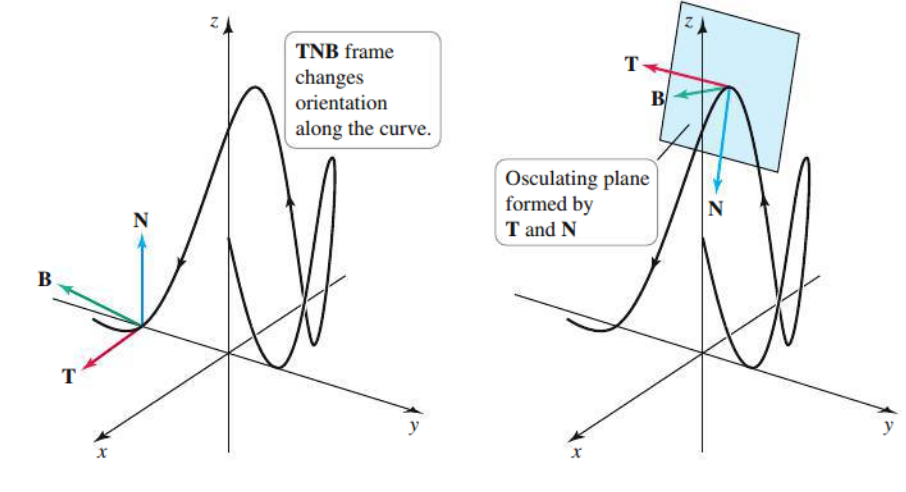
\includegraphics[width=0.6\linewidth]{images/briggs_14_05/fig14_37}
  \end{center}
  \vspace*{\stretch{1}}
  
  The coordinate system defined by these vectors is called the \textbf{TNB frame}. The rate at which the curve $C$ twists out of the plane is the rate at which $\vecB$ changes as we move along $C$, which is $\ds\frac{d\vecB}{ds}$.

  \begin{align*}
    \frac{d\vecB}{ds}&= \frac{d}{ds}\parens{\vecT\times\vecN}
      =\underbrace{\frac{d\vecT}{ds}\times\vecN}_\bfO+\vecT\times \frac{d\vecN}{ds}
      =\vecT\times \frac{d\vecN}{ds}
  \end{align*}
  \vspace*{\stretch{1}}

  $\ds\frac{d\vecB}{ds}$ is:
  \begin{tasks}[label=\textbullet](1)
    \task orthogonal to both $\vecT$ and $\ds\frac{d\vecN}{ds}$,
    \task orthogonal to $\vecB$ (Theorem 14.2),
    \task parallel with $\vecN$.
  \end{tasks}
  \pagebreak

  Since $\ds\frac{d\vecB}{ds}$ is parallel to $\vecN$, we write
    \[\frac{d\vecB}{ds}=-\tau\vecN\]
  where $\tau$ is the \textit{torsion} (the negative sign is conventional). We can solve for $\tau$ via the dot product:
  \begin{align*}
    \frac{d\vecB}{ds}\cdot\vecN=-\tau \underbrace{\vecN\cdot\vecN}_1 \quad\Longrightarrow\quad
    \frac{d\vecB}{ds}\cdot\vecN=-\tau
  \end{align*}
  \vspace*{\stretch{1}}

  \begin{defn*}[Unit Binormal Vector and Torsion]
    Let $C$ be a smooth parameterized curve with unit tangent and principal unit normal vectors $\vecT$ and $\vecN$, respectively. Then at each point of the curve at which the curvature is nonzero, the \textbf{unit binomial vector} is
      \[\vecB=\vecT\times\vecN,\]
    and the \textbf{torsion} is
      \[\tau=-\frac{d\vecB}{ds}\cdot\vecN\]
  \end{defn*}
  \vspace*{\stretch{1}}
  \pagebreak

  \begin{ex*}
    Consider the circle $C$ defined by
      \[\vecr(t)=\bracket{R\cos(t),\,R\sin(t)}, \textnormal{ for }0\leq t\leq 2\pi,\textnormal{ with }R>0.\]
    Find the unit binormal vector $\vecB$ and determine the torsion.
  \end{ex*}
  \vspace*{\stretch{1}}

  \begin{ex*}
    Compute the torsion of the helix
      \[\vecr(t)=\bracket{a\cos(t),\,a\sin(t),\,bt}, \textnormal{ for }t\geq 0,\textnormal{ and }b>0.\]
  \end{ex*}
  \vspace*{\stretch{1}}

  \pagebreak
  \vspace*{\stretch{1}}

  \noindent
  \fbox{\parbox{0.9875\linewidth}{
    \TabPositions{0.35\linewidth}
    \textbf{Summary: Formula for Curves in Space}\\
    Position function: \tab $\vecr(t)=\bracket{x(t),\,y(t),\,z(t)}$\\[\baselineskip]
    Velocity: \tab $\vecv=\vecr'$\\[\baselineskip]
    Acceleration: \tab $\veca=\vecv'$\\[\baselineskip]
    Unit tangent vector: \tab $\ds\vecT=\frac{\vecv}{\abs{\vecv}}$\\[\baselineskip]
    Principal unit normal vector: \tab $\ds\vecN=\frac{d\vecT/dt}{\abs{d\vecT/dt}}$ (provided $d\vecT/dt\neq \bfO$)\\[\baselineskip]
    Curvature: \tab $\ds\kappa=\abs{\frac{d\vecT}{ds}}=\frac{1}{\abs{\vecv}}\abs{\frac{d\vecT}{dt}}=\frac{\abs{\vecv\times\veca}}{\abs{\vecv}^3}$\\[\baselineskip]
    Components of acceleration: \tab $\veca=a_N\vecN+a_T\vecT$, where\\[\baselineskip]
    \mbox{}\tab $\ds a_N=\kappa\abs{\vecv}^2=\frac{\abs{\vecv\times\veca}}{\abs{\vecv}}$ and $\ds a_T=\frac{d^2s}{dt^2}=\frac{\vecv\cdot\veca}{\vecv}$\\[1.5\baselineskip]
    Unit binormal vector: \tab $\ds\vecB=\vecT\times\vecN=\frac{\vecv\times\veca}{\abs{\vecv\times\veca}}$\\[\baselineskip]
    Torsion: \tab $\ds\tau=-\frac{d\vecB}{ds}\cdot\vecN=\frac{\parens{\vecv\times\veca}\cdot\veca'}{\abs{\vecv\times\veca}^2}=\frac{\parens{\vecr'\times\vecr''}\cdot\vecr'''}{\abs{\vecr'\times\vecr''}^2}$
  }}
  \vspace*{\stretch{1}}

  \pagebreak
  
\end{document}
